%Version 3.1 December 2024
% See section 11 of the User Manual for version history
%
%%%%%%%%%%%%%%%%%%%%%%%%%%%%%%%%%%%%%%%%%%%%%%%%%%%%%%%%%%%%%%%%%%%%%%
%%                                                                 %%
%% Please do not use \input{...} to include other tex files.       %%
%% Submit your LaTeX manuscript as one .tex document.              %%
%%                                                                 %%
%% All additional figures and files should be attached             %%
%% separately and not embedded in the \TeX\ document itself.       %%
%%                                                                 %%
%%%%%%%%%%%%%%%%%%%%%%%%%%%%%%%%%%%%%%%%%%%%%%%%%%%%%%%%%%%%%%%%%%%%%

%%\documentclass[referee,sn-basic]{sn-jnl}% referee option is meant for double line spacing

%%=======================================================%%
%% to print line numbers in the margin use lineno option %%
%%=======================================================%%

%%\documentclass[lineno,pdflatex,sn-basic]{sn-jnl}% Basic Springer Nature Reference Style/Chemistry Reference Style

%%=========================================================================================%%
%% the documentclass is set to pdflatex as default. You can delete it if not appropriate.  %%
%%=========================================================================================%%

%%\documentclass[sn-basic]{sn-jnl}% Basic Springer Nature Reference Style/Chemistry Reference Style

%%Note: the following reference styles support Namedate and Numbered referencing. By default the style follows the most common style. To switch between the options you can add or remove �Numbered� in the optional parenthesis. 
%%The option is available for: sn-basic.bst, sn-chicago.bst%  
 
%%\documentclass[pdflatex,sn-nature]{sn-jnl}% Style for submissions to Nature Portfolio journals
%%\documentclass[pdflatex,sn-basic]{sn-jnl}% Basic Springer Nature Reference Style/Chemistry Reference Style
\documentclass[pdflatex,sn-mathphys-num]{sn-jnl}% Math and Physical Sciences Numbered Reference Style
%%\documentclass[pdflatex,sn-mathphys-ay]{sn-jnl}% Math and Physical Sciences Author Year Reference Style
%%\documentclass[pdflatex,sn-aps]{sn-jnl}% American Physical Society (APS) Reference Style
%%\documentclass[pdflatex,sn-vancouver-num]{sn-jnl}% Vancouver Numbered Reference Style
%%\documentclass[pdflatex,sn-vancouver-ay]{sn-jnl}% Vancouver Author Year Reference Style
%%\documentclass[pdflatex,sn-apa]{sn-jnl}% APA Reference Style
%%\documentclass[pdflatex,sn-chicago]{sn-jnl}% Chicago-based Humanities Reference Style

%%%% Standard Packages
%%<additional latex packages if required can be included here>

\usepackage{graphicx}%
\usepackage{multirow}%
\usepackage{amsmath,amssymb,amsfonts}%
\usepackage{amsthm}%
\usepackage{mathrsfs}%
\usepackage[title]{appendix}%
\usepackage{xcolor}%
\usepackage{textcomp}%
\usepackage{manyfoot}%
\usepackage{booktabs}%
\usepackage{algorithm}%
\usepackage{algorithmicx}%
\usepackage{algpseudocode}%
\usepackage{listings}%
%%%%

%%%%%=============================================================================%%%%
%%%%  Remarks: This template is provided to aid authors with the preparation
%%%%  of original research articles intended for submission to journals published 
%%%%  by Springer Nature. The guidance has been prepared in partnership with 
%%%%  production teams to conform to Springer Nature technical requirements. 
%%%%  Editorial and presentation requirements differ among journal portfolios and 
%%%%  research disciplines. You may find sections in this template are irrelevant 
%%%%  to your work and are empowered to omit any such section if allowed by the 
%%%%  journal you intend to submit to. The submission guidelines and policies 
%%%%  of the journal take precedence. A detailed User Manual is available in the 
%%%%  template package for technical guidance.
%%%%%=============================================================================%%%%

%% as per the requirement new theorem styles can be included as shown below
\theoremstyle{thmstyleone}%
\newtheorem{theorem}{Theorem}%  meant for continuous numbers
%%\newtheorem{theorem}{Theorem}[section]% meant for sectionwise numbers
%% optional argument [theorem] produces theorem numbering sequence instead of independent numbers for Proposition
\newtheorem{proposition}[theorem]{Proposition}% 
%%\newtheorem{proposition}{Proposition}% to get separate numbers for theorem and proposition etc.

\theoremstyle{thmstyletwo}%
\newtheorem{example}{Example}%
\newtheorem{remark}{Remark}%

\theoremstyle{thmstylethree}%
\newtheorem{definition}{Definition}%

\raggedbottom
%%\unnumbered% uncomment this for unnumbered level heads

\begin{document}

\title[Article Title]{P7. Analyzing Thematic Alignment in Scientific Journals}

%%=============================================================%%
%% GivenName	-> \fnm{Joergen W.}
%% Particle	-> \spfx{van der} -> surname prefix
%% FamilyName	-> \sur{Ploeg}
%% Suffix	-> \sfx{IV}
%% \author*[1,2]{\fnm{Joergen W.} \spfx{van der} \sur{Ploeg} 
%%  \sfx{IV}}\email{iauthor@gmail.com}
%%=============================================================%%

\author{\fnm{Roberto} \sur{Antoniello 47891A}} 

%%==================================%%
%% Sample for unstructured abstract %%
%%==================================%%

\abstract{This project focuses on quantitatively assessing whether articles published in a specific journal align with its stated "Aims \& Scope". The core objective is therefore to evaluate wheter the journal's content remains consistent with its declared scope over time. The chosen journal for the demonstration is "Frontiers in Artificial Intelligence".

To achieve this, article abstracts are represented through sentence embeddings generated using a domain-specific pre-trained model based on Sentence-BERT. The Aim \& Scope text is encoded using the same model and it is used as ground truth. Cosine similarity is computed between each abstract embedding and the scope embedding to obtain an alignment score.

Descriptive statistics and temporal aggregation are employed to analyze the distribution of alignment scores and to detect potential thematic drift across publication years.

The results provide a quantitative framework for assessing coherence between articles and scope in a scientific journal using semantic similarity measures. }

%%================================%%
%% Sample for structured abstract %%
%%================================%%

% \abstract{\textbf{Purpose:} The abstract serves both as a general introduction to the topic and as a brief, non-technical summary of the main results and their implications. The abstract must not include subheadings (unless expressly permitted in the journal's Instructions to Authors), equations or citations. As a guide the abstract should not exceed 200 words. Most journals do not set a hard limit however authors are advised to check the author instructions for the journal they are submitting to.
% 
% \textbf{Methods:} The abstract serves both as a general introduction to the topic and as a brief, non-technical summary of the main results and their implications. The abstract must not include subheadings (unless expressly permitted in the journal's Instructions to Authors), equations or citations. As a guide the abstract should not exceed 200 words. Most journals do not set a hard limit however authors are advised to check the author instructions for the journal they are submitting to.
% 
% \textbf{Results:} The abstract serves both as a general introduction to the topic and as a brief, non-technical summary of the main results and their implications. The abstract must not include subheadings (unless expressly permitted in the journal's Instructions to Authors), equations or citations. As a guide the abstract should not exceed 200 words. Most journals do not set a hard limit however authors are advised to check the author instructions for the journal they are submitting to.
% 
% \textbf{Conclusion:} The abstract serves both as a general introduction to the topic and as a brief, non-technical summary of the main results and their implications. The abstract must not include subheadings (unless expressly permitted in the journal's Instructions to Authors), equations or citations. As a guide the abstract should not exceed 200 words. Most journals do not set a hard limit however authors are advised to check the author instructions for the journal they are submitting to.}


%%\pacs[JEL Classification]{D8, H51}

%%\pacs[MSC Classification]{35A01, 65L10, 65L12, 65L20, 65L70}

\maketitle

\section{Introduction}\label{sec1}

The continuous growth of scientific production leads to the problem of having systematic methods to evaluate and organize scholarly content efficiently. Academic journals define their thematic boundaries through the Aim \& Scope section, which specifies the topics and research directions considered relevant within their editorial framework.

Maintaining coherence between published articles and the declared scope is essential for preserving the journal's identity.
Typically this coherence is assessed qualitatively, relying on editorial judgment rather than quantitative evidence.
\\ \\
This project proposes a quantitative framework which measures the semantic alignment between published articles and the journal's Aim \& scope. Texts are represented as semantic vectors using transformer-based sentence embeddings.
The editorial mission is encoded as a reference vector(our ground truth) within the same semantic space. Cosine similarity is computed between each article abstract and the reference vector, thus producing an alignment score.
\\ \\
The distribution of similarity scores enables the evaluation of thematic consistency and the analysis of potential thematic drift across publication years.
The main goal is to quantify the average alignment and examine the statistical behavior of similarity scores in order to assess editorial coherence over time.

\section{Dataset}\label{sec2}

The dataset consists of a collection of scientific articles obtained from a single academic journal. The chosen journal is Frontiers in Artificial Intelligence. The first step was obtaining the ISSN identifier of the journal and the articles were then extracted using the Crossref API. The chosen range of time spans five years, including all the articles published between January 2021 and December 2025.\\\\
Each record includes the following fields:

\begin{itemize}
\item title
\item abstract
\item doi (digital object identifier)
\end{itemize}
These fields provide a representation of the article content. The corpus consists of 1530 articles, which is enough to produce a meaningful distribution of similarity scores and support statistical analysis.


\section{Methodology}\label{sec3}

The proposed approach is based on a semantic analysis pipeline designed to measure the alignment between scientific articles of the chosen journal and its declared Aim \& Scope.


The pipeline is built as follow by four stages:
\begin{enumerate}
\item text preprocessing
\item embedding generation
\item similarity computation
\item Temporal aggregation and drift analysis
\end{enumerate}

\subsection{text preprocessing}\label{subsec2}

Before generating embeddings, a data cleaning phase is applied. This initial step includes the normalization of whitespace and elimination of non-printable characters. No aggressive linguistic preprocessing is performed, as transformer-based models preserve semantic information more effectively when operating on minimally altered text.\\
BERT-based models are trained on natural language text and they need the full syntactic and semantic structure of sentences to construct meaningful representations.\\
So, applying aggressive preprocessing would degrade the quality of the resulting embeddings.\\\\
The final output of this phase is a cleaned textual corpus, where each abstract and the scope are represented as a single string. The corpus and the scope are then used as input for the embedding generation process.

\subsection{embedding generation}\label{subsec2}

The core of the methodology used in this project relies on transforming text into vector representations (embeddings).
A pre-trained Sentence-BERT model is used in order to accomplish this, which is \textbf{allenai-specter}. This model is fine-tuned on scientific papers using citation context as a supervision signal. Two papers linked by a citation are pushed closer together in the embedding space, while unrelated papers are pushed apart.\\
Each abstract is encoded into a fixed-dimensional vector. The Aim \& Scope text is encoded using the same model, generating an embedding that acts as a ground truth representation of the journal thematic focus.

\subsection{Similarity computation}\label{subsec4}

The quantification of the thematic alignment between each article and the declared scope is done by using cosine similarity.
This computation technique is applied between the abstract embeddings and the scope reference vector.\\
Let $\mathbf{a}_i$ be \textit{\textbf{i}}-th article and let $\mathbf{e}_{ai}$ and $\mathbf{e}_{scope}$ be the corresponding embeddings vector of the article and the journal scope. The following formula is the actual cosine similarity computed for each article involved.

{\large
\[
\text{score}(a_i) = \frac{\mathbf{e}_{a_i} \cdot \mathbf{e}_{scope}}{\|\mathbf{e}_{a_i}\| \cdot \|\mathbf{e}_{scope}\|}
\]
}
Cosine similarity is the cosine of the angle between the vectors; it is the dot product of the vectors divided by the product of their lengths. A value close to 1 indicates a high alignment score with the scope; a value close to 0 indicates thematic distance. Negative values are theoretically possible but unlikely in this context given the shared domain.

\subsection{Temporal aggregation and drift analysis}\label{subsec5}

Once a score is assigned to each article, the distribution of alignment scores is analyzed both globally and longitudinally. Per-year aggregation is computed by grouping articles by publication year and calculating the mean and standard deviation of scores within each group. This temporal view allows the detection of potential thematic drift, which is a systematic shift in the average alignment over time, as well as changes in score variance, which may reflect increasing editorial heterogeneity.

\section{Results}\label{sec4}

The global distribution of alignment across all articles tell us that the majority of publications has a high semantic alignment to the declared scope of the journal Frontiers in Artificial Intelligence.\\
As we can see in the tables below, the global mean is over 0.7 and the standard deviation has a value near to zero, which tell us that there's not a much dispersion around the mean. This result is confirmed even if we look at the values filtered by year.
\begin{table}[h]
\centering
\caption{Descriptive statistics of alignment score globally}
\label{tab:alignment_scores}
\begin{tabular}{lr}
\hline
\textbf{Metric} & \textbf{Value} \\ \hline
Mean                          & 0.727           \\
Standard deviation            & 0.065           \\
Minimum                       & 0.516           \\
Maximum                       & 0.907           \\ \hline 
\end{tabular}
\end{table}
\begin{table}[h]
\centering
\caption{Descriptive statistics of alignment scores by year}
\label{tab:alignment_year}
\begin{tabular}{cccc}
\hline
\textbf{Year} & \textbf{Mean} & \textbf{Std. Dev.} & \textbf{Articles per year} \\ \hline
2021          & 0.7079        & 0.0648             & 192                        \\
2022          & 0.7180        & 0.0611             & 276                        \\
2023          & 0.7326        & 0.0591             & 216                        \\
2024          & 0.7286        & 0.0689             & 292                        \\
2025          & 0.7355        & 0.0661             & 554                        \\ \hline 
\end{tabular}
\end{table}
\begin{figure}[h]
    \centering
    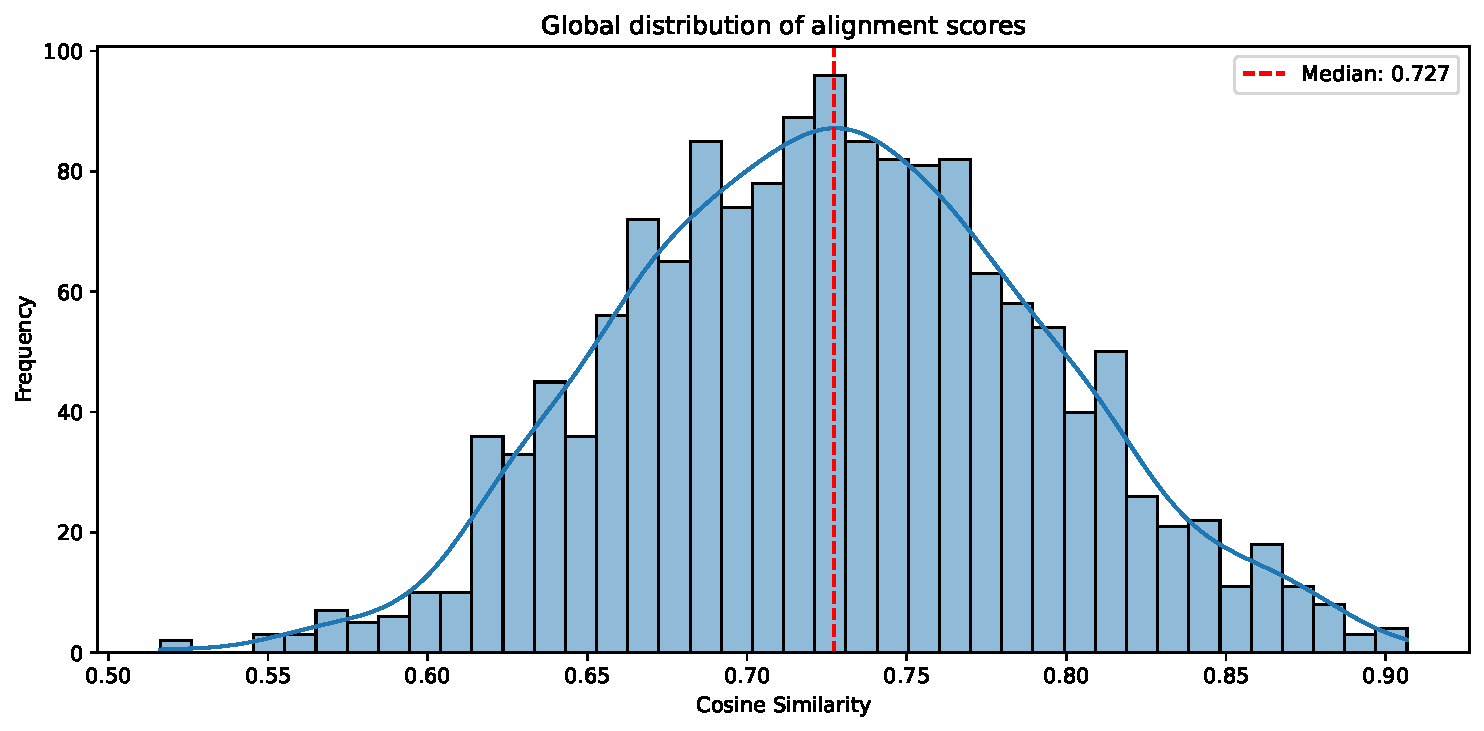
\includegraphics[width=0.85\textwidth]{global_distribution.pdf}
    \caption{Global distribution of alignment scores across the dataset.}
    \label{fig:global_distribution}
\end{figure}

Related to temporal analysis, the data provides insight about a possible thematic drift over time.\\
The mean value score increases slightly from 0.7079 in 2021 to 0.7355 in 2025, showing a slight and gradual increase in alignment to the Journal's scope over time. The standard deviation remains relatively stable year by year (0.0591 - 0.0689), with a slight increase in variance in more recent years.\\
This result suggests this Journal maintains a stable editorial coherence, with no single year exhibiting unusually high variance in alignment.\\
These obtained data are limited to the selected 2021-2025 time window. A broader analysis would be required to assess whether this pattern holds across older and earlier publication years.

\begin{figure}[h]
    \centering
    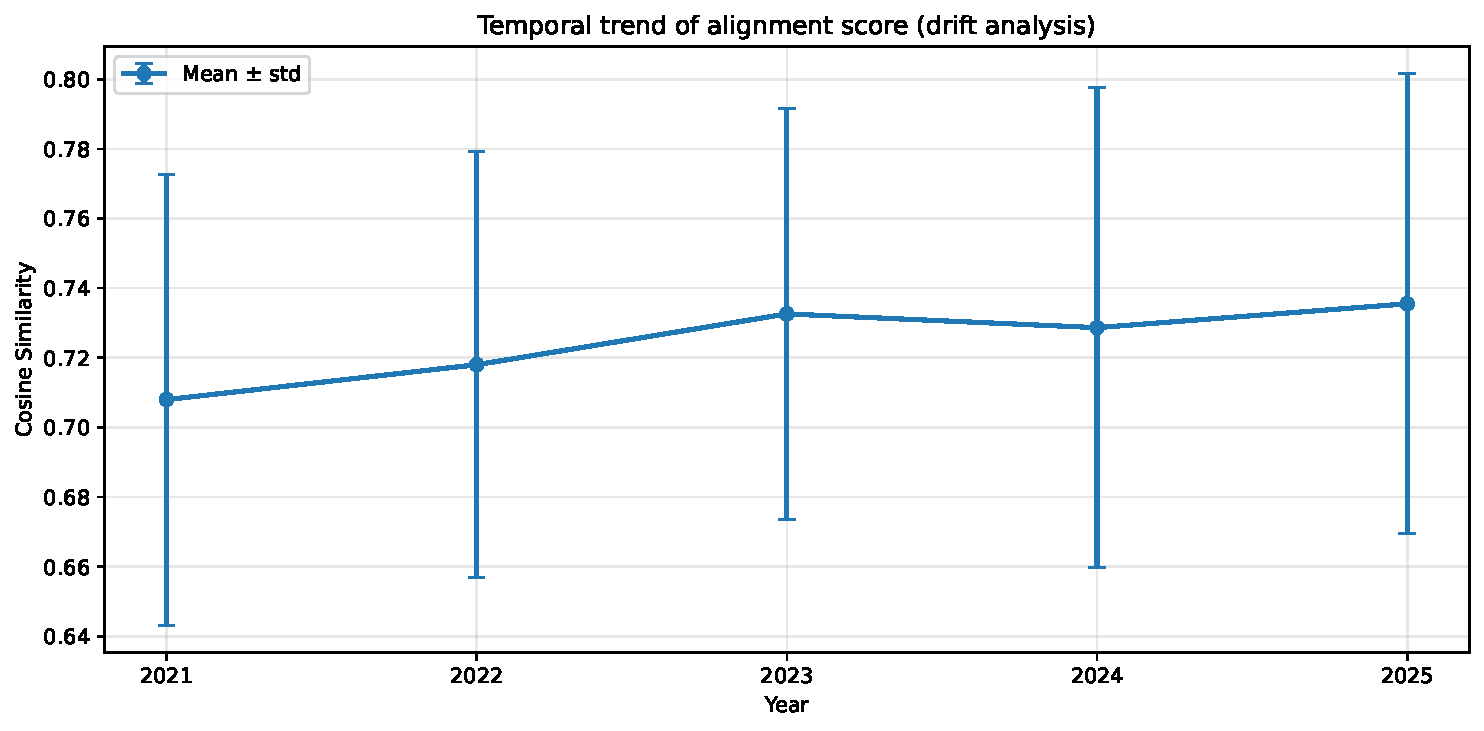
\includegraphics[width=0.85\textwidth]{temporal_trend_alignment.pdf}
    \caption{Temporal trend of alignment score from january 2021 to december 2025.}
    \label{fig:global_distribution}
\end{figure}


Extremely low scores represent articles that are less aligned with the journal scope, while high scores close to 0.9 indicate very strong semantic alignment. Overall the analysis confirms that the journal consistently publishes articles coherent with its declared Aim \& Scope, with a small number of publications deviating from this focus.


\section{Conclusion}\label{sec5}

This project introduced a quantitative framework to assess the alignment between scientific publications and the declared scope of a journal. By using semantic similarity techniques, each article was mapped to a continuous alignment score, enabling a systematic and reproducible evaluation process.\\
In this case study, results showed that Frontiers in Artificial Intelligence maintains a high thematic coherence across the 2021 - 2025 period. The global distribution of scores is concentrated around the mean with limited dispersion. This means most publications are consistently aligned with the declared scope, while a small subset deviates from it.\\
The main contribution of this project is the introduction of a normalized metric that enables comparison across time, by formalizing the scope alignment as a measurable quantity.\\

\section*{Declarations}
\textbf{Ai Usage Disclaimer:} parts of this project have been realized with the assistance of ChatGPT(model GPT-5.3) and Claude(model Sonnet 4.6) for the following types of tasks:
\begin{itemize}
\item Reviewing and drafting text during the writing of this report.
\item Collecting ideas about results analysis.
\item Generation of Python code to support the development.
\end{itemize}

Every content generated by AI has been reviewed and tested by a human.
\begin{thebibliography}{9}

\bibitem{reimers2019}
N. Reimers and I. Gurevych,
\textit{Sentence-BERT: Sentence Embeddings using Siamese BERT-Networks},
In Proceedings of the 2019 Conference on Empirical Methods in Natural Language Processing and the 9th International Joint Conference on Natural Language Processing (EMNLP-IJCNLP), pp. 3982--3992, 2019.

\bibitem{picascia2025}
S. Picascia, S. Montanelli, S. Salini, S., \& Verzillo, S. (2025).
\textit{The Atlas of Data Science Research},
IEEE Access, 2025.

\end{thebibliography}

\end{document}
